%%
% Please see https://bitbucket.org/rivanvx/beamer/wiki/Home for obtaining beamer.
%%
\documentclass[aspectratio=169]{beamer}
\usetheme{Antibes}
\usepackage{xcolor}
\mode<presentation>

\useoutertheme{miniframes} 
\useinnertheme{circles}

\definecolor{primary}{HTML}{003469}
\definecolor{secondary}{HTML}{003469}
\definecolor{tertiary}{HTML}{00addc}


\setbeamercolor{titlelike}{bg=white,fg=primary}

\setbeamercolor{palette primary}{bg=tertiary,fg=white}
\setbeamercolor{palette secondary}{bg=tertiary,fg=white}
\setbeamercolor{palette tertiary}{bg=secondary,fg=white}
\setbeamercolor{structure}{fg=secondary} % itemize, enumerate, etc
\setbeamercolor{section in toc}{fg=secondary} % TOC sections
% Override palette coloring with secondary
\setbeamercolor{subsection in head/foot}{bg=tertiary,fg=white}
\usepackage{natbib}
\bibliographystyle{unsrtnat}
\setcitestyle{authoryear,open={(},close={)}}
\usepackage{csquotes}
\usepackage{hyperref}

\hypersetup{
    colorlinks=true,
    linkcolor=black,
    filecolor=black,      
    urlcolor=cyan,
    pdftitle={Python, Cloud and Automation for TE: 3. Automation, Cloud and Examples},
    }



\title{\large{\textbf{Python, Cloud and Automation}} \newline\newline 3. Automation, Cloud and Examples}

\author{Jack Minchin}
\institute{Tourism Economics}
\date{2022}

\begin{document}

\frame{\titlepage}

\begin{frame}
\frametitle{Table of Contents}
\tableofcontents
\end{frame}


\section{Cloud Technologies}

\begin{frame}{What are cloud solutions?}

\begin{itemize}
	\item At the most basic level, cloud computing is the ability to access computers that are not on local premises. 
	\item In practise, cloud technology is an umbrella term for a variety of different computing services (file storage, compute, Platform as a Service (PaaS), cloud functions and pipelines)
	\item There are a number of cloud providers, at OE we have access to Azure and AWS. Azure is my preferred choice because of its integration with Active Directory (Microsoft) and the more verbose naming conventions (Azure App Service vs. AWS Elastic Beanstalk)
\end{itemize}

\end{frame}

\begin{frame}{Pipelines}

\begin{itemize}
	\item Pipelines are automated tasks that run in the cloud they can be triggered by pushing to a git repository, or through an API call.
	\item There are number of providers that offer pipelines but I have been using CircleCI because of their free tier. 
\end{itemize}
\end{frame}

\section{Example 1: Whitbread}

\begin{frame}{Example 1: Whitbread Outputs (Basic)}

\begin{itemize}
	\item Whitbread take a very basic quarterly breakdown of some GTS and Macro model indicators.
	\item The process is:
	\begin{enumerate}
		\item Run the macro and GTS extract
		\item Update the links in the model file
		\item Copy the output sheets into a new workbook. 
		\item Break links and save.
	\end{enumerate}
	\item Manual process time 40 minutes - 1 hour.
\end{itemize}
\end{frame}

\begin{frame}{Creating a pipeline}

\begin{figure}
\centering
	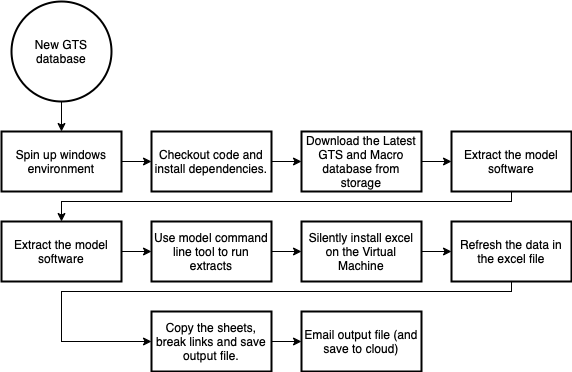
\includegraphics[width=0.7\linewidth]{graphics/WhitbreadPipeline.png}
\end{figure}	


\end{frame}



\begin{frame}{Languages \& Technologies Used}

\begin{itemize}
	\item Python - for running some of the orchestration
	\item PowerShell - Interacting with Windows \& Excel
	\item Azure Storage - storing the database files
	\item Git - Managing the project and codebase
	\item CircleCI YAML - Writing the pipelines steps
\end{itemize}	

\begin{block}{Time saving}
	\textbf{Manual method:} 1 hour. \newline
	\textbf{Pipeline method:} 8 minutes
\end{block}


\end{frame}


\section{Example 2: Country Reports}

\begin{frame}{Example 2: Country Report Generation (Advanced)}

\begin{itemize}
	\item The country report generator create $\sim$ 40 PDF reports with text and plots. 
	\item The manual process:
	\begin{enumerate}
		\item Creation of input file.
		\item Load excel file for each report.
		\item Update the links in each excel file.
		\item Rewrite boiler plate text to reflect new data.
		\item Fix plots where necessary.
		\item Write custom commentary.
		\item Save to PDF.
	\end{enumerate}
\end{itemize}

\end{frame}

\begin{frame}{Creating a pipeline}
\begin{figure}
\centering
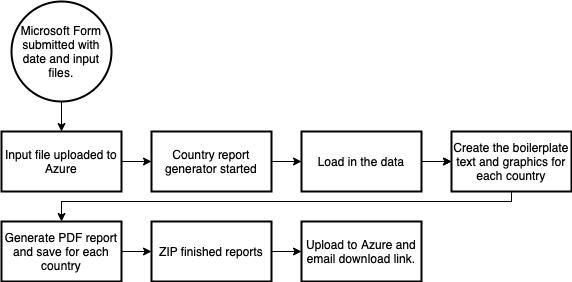
\includegraphics[width=0.7\linewidth]{graphics/CountryReportGenerator.drawio.png}	
\end{figure}

\end{frame}

\begin{frame}{Languages \& Technologies Used}
\begin{itemize}
	\item Python - for orchestration, creating text and plots.
	\item Azure Storage - storing the input and output files
	\item Azure Functions - triggering the process when a new input file is added.
	\item Node.JS - application architecture and PDF generation.
	\item Git - Managing the project and codebase
	\item CircleCI YAML - Writing the pipelines steps.
\end{itemize}	

\begin{block}{Time saving}

\textbf{Manual method:} 3 people 3 days. \newline
\textbf{Pipeline method:} 10 minutes + time to write custom text (1 day?).

\end{block}
\end{frame}

\section{Example 3: SweRe}

\begin{frame}{Sweden Regional TSA PowerPoints}

\begin{itemize}
	\item Creation of 8 regional TSA reports in PowerPoint. The text and graphics are entirely boilerplate. 
	\item Using Python and a package called python-pptx, the code takes the regular output from the Excel model file and outputs the reports in .pptx and PDF.
	\begin{block}{Time saving}

\textbf{Manual method:} Multiple days \newline
\textbf{Pipeline method:} 40 seconds

\end{block}
\end{itemize}
	
\end{frame}

\section{Example 4: APF}

\begin{frame}{APF IATA Data Inputs}

\begin{itemize}
 	\item We receive a monthly 2020 - To Date data file for PAX and RPK figures from IATA. 
 	\item It is in a long form structure with full country names.
 	\item Process:
 	\begin{enumerate}
 		\item Receive input files
 		\item Convert to wide form, change country names to model codes.
 		\item Extrapolate to the end of the current quarter.
 		\item Export readin file for model.	
 	\end{enumerate}
 	\item Uses Python notebooks.

\end{itemize}
	
\end{frame}


\begin{frame}{APF Automated Checks}

\begin{itemize}
	\item The number of variables in the APF model mean that it is impossible to check each variable series manually.
	\item We can load an extract from APF and automatically run tests, e.g:
	\begin{enumerate}
	\item Ensure no negative values.
	\item Ensure that current release is with $x \%$ of previous release.
	\item Ensure that PAXALL (sum of bilateral indicators) is not greater than PAX (total pax from IATA)
	\end{enumerate}
	\end{itemize}

	
\end{frame}





	




\end{document}
